\begin{slide}
\pagestyle{headings}
\sf
\header{Consistency of measurements}
\Large
Example: Two measurements $y_1$ and $y_2$ with errors
$\sigma_1$ and $\sigma_2$; the true value $a$ is known,
are the measurements consistent with $a$?:
%
\begin{figure}[h]
\unitlength1cm
  \begin{picture}(8,6.2)
    \put(0.,0.4){\epsfig{file=feynman/lco1.ps,width=5.5cm}}
    \put(8.,0.4){\epsfig{file=feynman/lco2.ps,width=5.5cm}}
    \put(1.,0.){
$\chi^2 = \frac{(y_1 - a)^2}{\sigma_1^2} + 
            \frac{(y_2 - a)^2}{\sigma_2^2} = 2$}  
\put(10.,0.){$\chi^2 = 8$}
\end{picture}
\end{figure}
%
$\rightarrow \chi^2$ is a measure of the consistency
%
%\vspace{7mm}
\end{slide}
%




\begin{slide}
\pagestyle{headings}
\sf
\header{Consistency of measurements}
\Large
\underline{Expected probability density  for 
$\vec{y} = (y_1,y_2)$  (case $a=0; \sigma_1 = \sigma_2 = \sigma$):}
\begin{figure}[h]
\unitlength1cm
  \begin{picture}(8,6.)
    \put(-.6,0.){\epsfig{file=feynman/lco3.ps,width=6.2cm}}
%\put(6.,5.){$ L(\vec{y},a) \propto
%e^{-y_1^2/2} e^{-y_2^2/2} 
%\sim e^{-\chi^2/2}
%$}
\put(5.,5.3){\Large
\begin{minipage}[t]{10cm}
\[
\begin{array}{l}
{\blue f(\vec{y})} \,  dy_1 dy_2 = 
\frac{ 1}{2\pi} e^{-y_1^2/2} e^{-y_2^2/2} \, dy_1 dy_2\\[2mm]  
= {\blue \frac{1}{2\pi} e^{-r^2/2}}\, dy_1 dy_2 \quad
\mbox{with}\; r=\sqrt{y_1^2+y_2^2}\\[4mm]
 {\blue f(r)} \, dr = \frac{2\pi r}{2\pi} r e^{-r^2/2} \, dr =  {\blue r e^{-r^2/2} }\, dr\\[4mm]
\chi^2 = r^2 \rightarrow \\[2mm] 
{\blue    f(\chi^2)} \, d\chi^2 = {\blue \frac{ 1}{2} e^{-\chi^2/2}} \, d\chi^2\\
\end{array}
\]
\end{minipage}
} 
\end{picture}
\end{figure}
\vspace*{-1mm}
$\rightarrow$ introduces $\chi^2$-distr. for $z=\chi^2$ and two 
dimensions (ndf=2):
$f(z,2) = \frac{1}{2}  e^{-z/2}$
%Trafo $L(\vec{y},a) \rightarrow$ prob. density $f(\chi^2)$\\
%General result for $n$ measurements: $\chi^2$ fct. for n-degrees of freedom
%\[ \rightarrow f(\chi^2,n) = 
%\frac{1}{\Gamma(n/2)2^{n/2}} \cdot
%(\chi^2)^{n/2-1} \cdot e^{-\chi^2/2}
%\]
%
\end{slide}


\begin{slide}
\pagestyle{headings}
\sf
\header{$\chi^2$-function for $n$ degrees of freedom}
\begin{figure}[h]
\unitlength1cm
  \begin{picture}(8,6.)
    \put(-1.3,0.){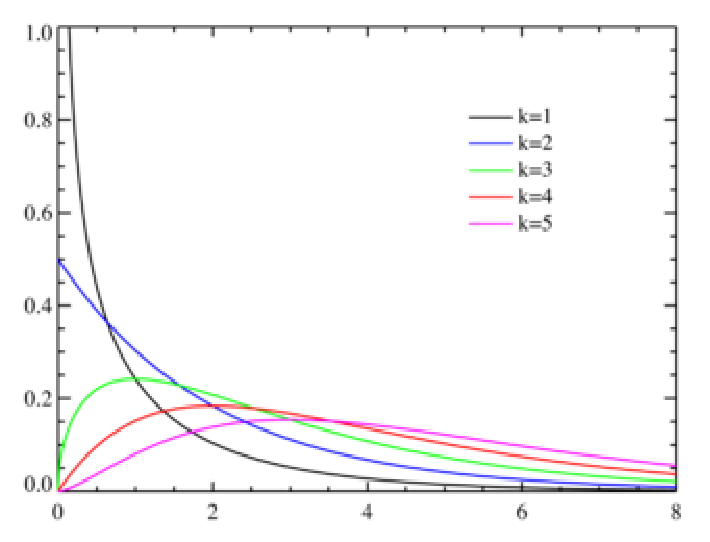
\epsfig{file=feynman/325px-Chi-square_distributionPDF.ps,
width=8.cm}}
\put(7.,5.){\Large
$f(\chi^2,n) = 
\frac{1}{\Gamma(n/2)2^{n/2}} \cdot
(\chi^2)^{n/2-1} \cdot e^{-\chi^2/2}$
}
\put(7.,4.){\Large with $\Gamma(n/2) 
= \int_{0}^{\infty} dt e^{-t} t^{n/2-1}$
}
\put(7.,3.){\framebox{
\begin{minipage}[t]{7.5cm}
\Large
%Es gilt:\\
$\int_0^{\infty} f(\chi^2,n) d\chi^2 = 1$\\[2mm]
$\langle \chi^2 \rangle = n$\\[2mm]
$V(\chi^2) = 2n; \; \sigma(\chi^2) = 
\sqrt{2n}$\\[2mm]
$\rightarrow \langle \chi^2/n \rangle = 1$\\[2mm] 
$\sigma(\chi^2/n) = \sqrt{2/n}$
\end{minipage}
}
}
\end{picture}
\end{figure}
%\vfill
%\vspace*{-5mm}
%Transformation $L(\vec{y},a) \rightarrow$ prob. density $f(\chi^2)$\\
%General result for $n$ measurements: $\chi^2$ fct. for n-degrees of freedom
%
%
\end{slide}



\begin{slide}
\Large
\pagestyle{headings}
\sf
\header{$\chi^2$-fit probability}
%
\underline{Common measure for consistency of measurements:}\\
Probability that for repeated experiments a  
$\chi^2\ge \chi^2_{actual}$ is
observed 
%
\[ prob(\chi^2,n) = \int_{\chi^2}^{\infty} f(\chi^2,n) d\chi^2
\quad \mbox{subst. } t = \chi^2/2
\]
\[ = \frac{1}{\Gamma(n/2)} \cdot \int_{\chi^2/2}^{\infty} 
dt\, e^{-t} \,t^{n/2-1} \]
%(available in CERNLIBS etc.)
%
\begin{figure}[h]
\unitlength1cm
  \begin{picture}(8,6.)
    \put(-1.3,0.){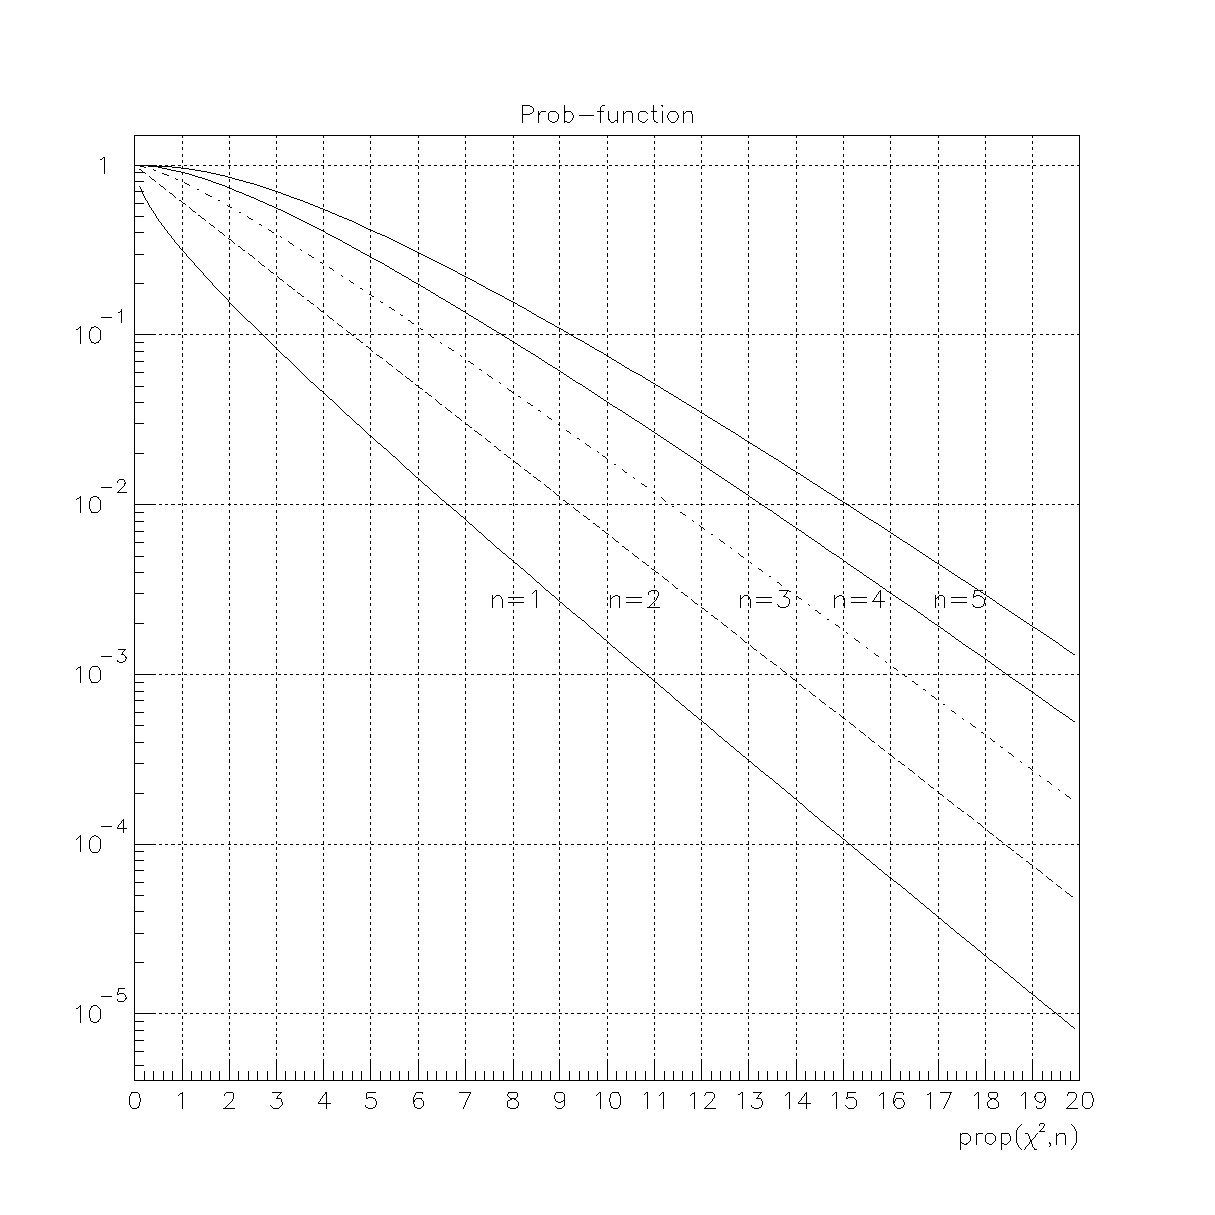
\epsfig{file=eps/probfct.eps,
width=7.cm}}
\put(-.5,1.){\large \red $prob(\chi^2,n)$ vs $\chi^2$ for various $n$}
\put(6.,3.){Add plot of expected flat distribution}
\end{picture}
\end{figure}
%
\end{slide}


\begin{slide}
\Large
\pagestyle{headings}
\sf
\header{$\chi^2$ for two measurements with unknown true value}
%
Until now the true value of $a$ was assumed to be known, 
%taken to be 
%known and used for $\chi^2$\\
%If $a$ is unknown $\rightarrow$ 
now replace by estimated $\hat{a}$;\\[2mm]
\underline{Example of two measurements:}
\begin{eqnarray*} 
\chi^2_{min} & = & 
\frac{ (y_1 - \hat{a})^2 } {\sigma_1^2} 
+
\frac{ (y_2 - \hat{a})^2 } {\sigma_2^2}
%;  
%\quad  \mbox{with} \quad G_i: = 1/\sigma_i^2 \\
\end{eqnarray*}
Using  the weighted average 
$\hat{a} = \frac{\dd G_1 y_1 + G_2 y_2}{\dd G_1+G_2}$ with $ \quad G_i: = 1/\sigma_i^2$ $\rightarrow$  
\end{slide}


\begin{slide}
\Large
\pagestyle{headings}
\sf
\header{$\chi^2$ for two measurements with unknown true value}
%
\vspace{-5mm}
\normalsize
\begin{eqnarray*}
\chi^2_{min} & = &   
  G_1 \cdot \left(y_1 - \frac{(G_1 y_1 + G_2 y_2)}{G_1+G_2} \right)^2 
+ G_2 \cdot \left(y_2 - \frac{(G_1 y_1 + G_2 y_2)}{G_1+G_2} \right)^2 \\
& = & 
  G_1 \cdot \left(\frac{(G_2 y_1 - G_2 y_2)}{G_1+G_2} \right)^2 
+ G_2 \cdot \left(\frac{(G_1 y_2 - G_1 y_1)}{G_1+G_2} \right)^2 \\
& = & 
\frac{G_1 G_2^2}{(G_1+G_2)^2} (y_1 -y_2)^2 + 
\frac{G_2 G_1^2}{(G_1+G_2)^2} (y_1 -y_2)^2 \\
& = & 
\frac{G_1 G_2 (G_1+G_2)}{(G_1+G_2)^2} \cdot  (y_1 -y_2)^2 
 =  \frac{G_1 \cdot G_2}{G_1+G_2} \cdot (y_1-y_2)^2\\ 
& = & 
\frac{1}{1/G_1 + 1/G_2} \cdot (y_1 - y_2)^2 
 = {  \pmb{  \frac{1}{\sigma_1^2+\sigma_2^2} \cdot 
(y_1-y_2)^2}} 
\end{eqnarray*}
\Large 
$\Delta = 
\frac{y_1 - y_2}{\sqrt{\sigma_1^2 +\sigma_2^2}}$ should follow
{\blue  \small \it (errorpropagation!)} 
gauss distribution $\sim e^{-\frac{\Delta^2}{2}}$\\[1mm]
$ \rightarrow$ $\chi^2 = \Delta^2$ follows \underline{1-dim} $\chi^2$
distr.!\\[1mm]
$\rightarrow$ One degree of freedom ``sacrificed'' for determination of
$\hat{a}$.\\[2mm]
\framebox{\begin{minipage}{12cm}
General: $n$-measurements with one unknown $a$\\ 
$\rightarrow$ follows $\chi^2$ distribution 
with $n-1$ degrees of freedom
\end{minipage}
}
\end{slide}


\begin{slide}
\Large
\pagestyle{headings}
\sf
\bheader{\darkgreen{Mini-exercise} Plot $\chi^2$ curves with computer}
%
\begin{figure}[h]
\unitlength1cm
  \begin{picture}(8,8.)
    \put(-1.3,0.){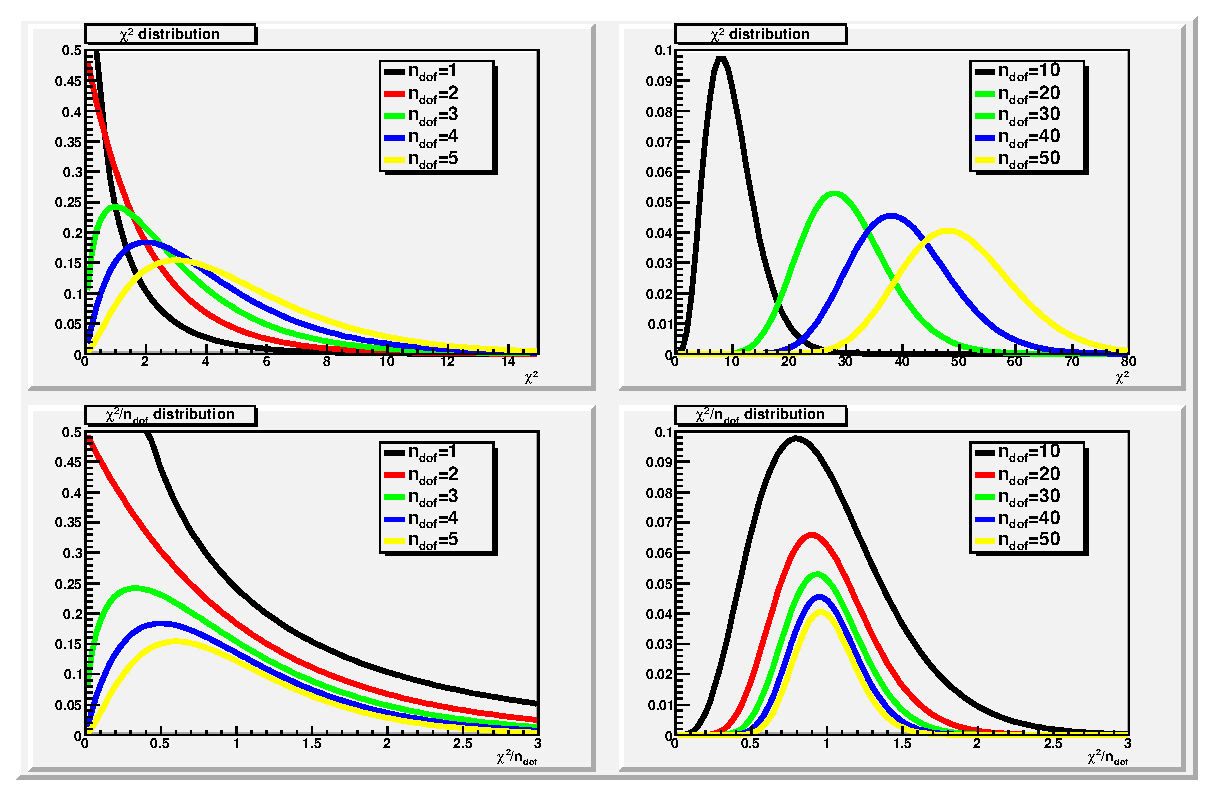
\epsfig{file=eps/chisq_ndf_curves.eps,width=12.cm}}
%    \put(-1.3,0.){\epsfig{file=prob_examples.ps,width=7.cm}}
\put(0.,-1.){\normalsize see  $/afs/desy.de/user/m/mgoebel/public/StatisticsWS/ChiSquareDistribution.C$}

%\put(-.5,1.){\large \red $prob(\chi^2,n)$ vs $\chi^2$ for various $n$}
%\put(6.,3.){Add plot of expected flat distribution}
\end{picture}
\end{figure}
%
\end{slide}

\begin{slide}
\Large
\pagestyle{headings}
\sf
\bheader{\darkgreen{Mini-exercise} Outlier rejection}
%
\begin{figure}[h]
\unitlength1cm
  \begin{picture}(8,8.)
    \put(2.,10.){\rotatebox{-90}{\epsfig{file=eps/average_mw_new.ps,width=8.cm}}}
%    \put(-1.3,0.){\epsfig{file=prob_examples.ps,width=7.cm}}

\put(0.,1.5){\normalsize see  $/afs/desy.de/user/m/mgoebel/public/StatisticsWS/AverageMW.C$}
\put(0.,1.){
\begin{minipage}[t]{14cm}
\darkgreen
Tasks: Determine weighted average, the $\chi^2_{min}$ and fit probability,
see what happens if one takes out the value with the largest deviation from the mean,
etc.
\end{minipage}
}
%\put(-.5,1.){\large \red $prob(\chi^2,n)$ vs $\chi^2$ for various $n$}
%\put(6.,3.){Add plot of expected flat distribution}
\end{picture}
\end{figure}
%
\end{slide}
